\chapter{Lasttests}

In diesem Abschnitt wurden Tests zur Belastbarkeit der Webanwendung durchgeführt. Dabei wurden die Ladezeiten des Systems 
geprüft, mit jeweils verschiedenen Anzahlen an parallel eingeloggten Benutzern und zur Verfügung gestellten Datenbankverbindungen.
Es wurde vier verschiedene Anzahlen an parallelen Sessions sowie zwei verschiedene Anzahlen an Datenbankverbindungen getestet. Dabei 
wurde von jeder Session über eine gemeinsame URL auf einen einzigen Server zugegriffen. Die Parallelität wurde unterteilt in 1, 5, 15 
und 20 gleichzeitig aktiven Benutzersessions. Die Tests wurden jeweils einmal mit zwei und einmal mit 10 zur Verfügung gestellten 
Datenbankverbindungen durchgeführt.

\section{Durchgeführte Tests}

\subsection{TestMeasurement}

\subsubsection{Beschreibung}

TestMeasurement beinhaltet, neben dem Ablauf, Variablen, welche die aktuelle Tageszeit auf dem Rechner in Millisekunden angibt, 
jeweils unmittelbar vor und nach einer zu testenden, durchgeführten Aktion. Durch Subtrahieren wird die Zeitspanne ermittelt und zur 
Auswertung auf der Konsole ausgegeben. Dieser Test wurde jeweils drei mal während den parallel laufenden Tests ausgeführt, um die 
verschiedenen Ladezeiten der jeweiligen Funktion zu messen.

\subsubsection{Ablauf}

Der Benutzer (in der Rolle eines Administrators) logged sich im System ein und führt eine Kurssuche durch, bei dem alle vorhandenen Kurse angezeigt werden. Der Kurs "Zweiter Test" wird angeklickt und auf dessen Detailseite meldet sich der Benutzer zu zwei Kurseinheiten ein, von denen er sich unmittelbar danach wieder abmeldet. Anschließend wird auf der Kurssuche-Seite nach dem Kurs "Yoga" geklickt und zu dessen Detailseite navigiert. Von dieser Seite geht der Benutzer über die Navigatinosleiste auf die Seite zur Seitenverwaltung und lässt sich bei der Nutzersuche alle registrierten Nutzer anzeigen. Daraufhin logged sich der Benutzer aus dem System aus.

\subsection{LoadTest}

\subsubsection{Beschreibung}

Der LoadTest wurde an bis zu 20 verschiedenen Rechnern durchgeführt. An jedem Rechner wurde genau eine .jar Datei ausgeführt, welche diesen Test beinhaltet. Dabei unterscheiden sich die Tests nur beim Beutzernamen und Passwort, um jeweils 1, 5, 15 und 20 
verschiedene Sessions zu simulieren.

\subsubsection{Ablauf}

Dieser Test beinhaltet zu einem Großteil den selben Ablauf wie TestMeasurement, es werden lediglich die Administratorfunktionen nicht durchgeführt, da der Benutzer keine Administratorrechte besitzt. Die Aktionen zwischen dem Login und Logout werden über eine for-Schleife 51 mal wiederholt.

\section{Diagramme}

In diesem Abschnitt werden beispielhaft zwei aussagekräftige Diagramme dargestellt, welche die Auswertung des Gesamtergebnisses und des Logins darstellen. Die y-Achse beschreibt die gemessenen Ladezeiten in Millisekunden, die x-Achse die Anzahl der parallel laufenden Nutzersessions.
Für die ermittelten Ergebnisse des TestMeasurement wurde jeweils ein Durchschnittswert erstellt und in einer Tabelle dokumentiert. Für die fünf ausgeführten Aktionen (Login, Suche nach allen Kursen, Anmelden zu einer Kurseinheit, Suche eines bestimmten Kurses und Suche nach allen registrierten Nutzern) wurde anschließend der Durchschnittswert in das jeweilige Diagramm eingetragen.

\begin{figure}[h]
\centering
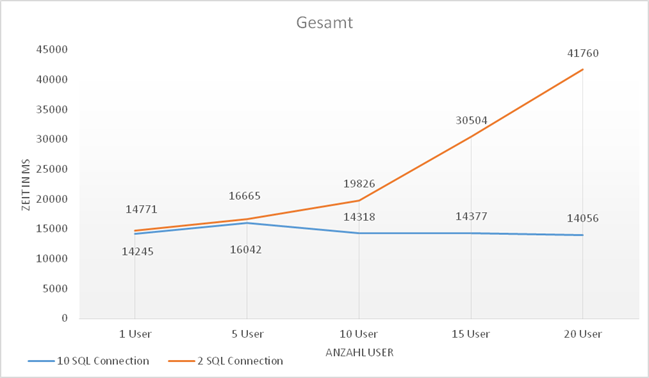
\includegraphics[width=0.7\linewidth]{img/gesamt}
\caption{Gesamtergebnis TestMeasurement}
\label{fig:TestMeasurement}
\end{figure}

\newpage

\begin{figure}[h]
\centering
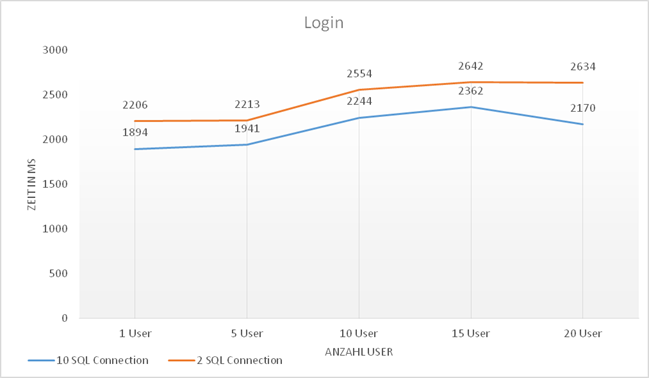
\includegraphics[width=0.7\linewidth]{img/login}
\caption{Gesamtergebnis Login}
\label{fig:Login}
\end{figure}

\section{Fazit der gesamten Auswertung}

Bei zehn zur Verfügung gestellten Datenbankverbindungen blieb die Auslastung des Systems, gemessen anhand der Ladezeit in Millisekunden und der Anzahl an parallel Aktiven Nutzersessions, beinahe gleichmäßig. Die Ladezeiten haben sich, entgegen der Erwartung, kaum verändert (was allerdings an und für sich für ein schnell reagierendes System spricht).
Bei zwei zur Verfügung gestellten Datenbankverbindungen stieg die Auslastung erwartungsgemäß exponentiell, aber nicht unverhältnismäßig negativ.
Anzumerken ist noch, dass die Ladezeiten beim Login sich nur geringfügig unterscheiden, unabhängig von der Anzahl der aktiven Benutzer oder Datenbankverbindungen.
Zusammenfassend lässt sich sagen, dass die Qualtitätsbestimmung aus dem Pflichtenheft bezüglich der Funktionalität die Ansprüche erfüllt. Bei zehn Datenbankverbindungen wird dieses Qualitätsmerkmal sogar überdurchschnittlich gut erreicht.